\documentclass[tikz, footheight=2em]{beamer}
\usetheme[hideothersubsections]{Hannover}
\usepackage[T1]{fontenc}
\usepackage[utf8]{inputenc}
\usepackage{amssymb}
\usepackage{amsthm}
\usepackage{amsmath}
\usepackage{color,graphicx}
\usepackage{ulem}
\usepackage{gensymb}
\usepackage{tikz}

\usecolortheme{dolphin}

\title{QAI Tetris}
\author{C.~Cousin, G.~Hondet, L.~Pineau, B.~Viry}
\date{}

\usetikzlibrary{patterns,arrows,positioning}
\tikzset{
    %Define standard arrow tip
    >=stealth',
    %Define style for boxes
    punkt/.style={
           rectangle,
           rounded corners,
           draw=black, very thick,
           text width=6.5em,
           minimum height=2em,
           text centered},
    % Define arrow style
    pildwn/.style={
           <-,
           thick,
           shorten <=2pt,
           shorten >=2pt,},
    pilup/.style={
           ->,
           thick,
           shorten <=2pt,
           shorten >=2pt,}
}

% ----------------------------------------------------------
% nuremotation des pages -----------------------------------
% ----------------------------------------------------------
\def\swidth{1.6cm}
\setbeamersize{sidebar width left=\swidth}
\setbeamertemplate{sidebar left}
{%
  {\usebeamerfont{title in sidebar}
    \vskip1.5em
    \usebeamercolor[fg]{title in sidebar}
    \insertshorttitle[width=\swidth,center,respectlinebreaks]\par
    \vskip1.25em
  }
  {
    \usebeamercolor[fg]{author in sidebar}
    \usebeamerfont{author in sidebar}
    \insertshortauthor[width=\swidth,center,respectlinebreaks]\par
    \vskip1.25em
  }
  \hbox to2cm{\hss\insertlogo\hss}
  \vskip1.25em
  \insertverticalnavigation{\swidth}
  \vfill
  \hbox to2cm{\hskip0.6cm\usebeamerfont{subsection in
      sidebar}\strut\usebeamercolor[fg]{subsection in
      sidebar}\insertframenumber /\inserttotalframenumber\hfill}
  \vskip3pt
}
% ----------------------------------------------------------


\begin{document}

\frame{\titlepage}

\AtBeginSection[]
{%
  \begin{frame}
    \frametitle{Plan}
    \tableofcontents[currentsection]
  \end{frame}
}

\section{Methode d'apprentissage}
\begin{frame}[t]{Apprentissage par renforcement}
  \begin{block}{Principe}
    Une entité évoluant dans son environnement se voit attribuées des
    récompenses en fonction de la pertinence de ses actions.
    \begin{figure}[h]
      \begin{center}
        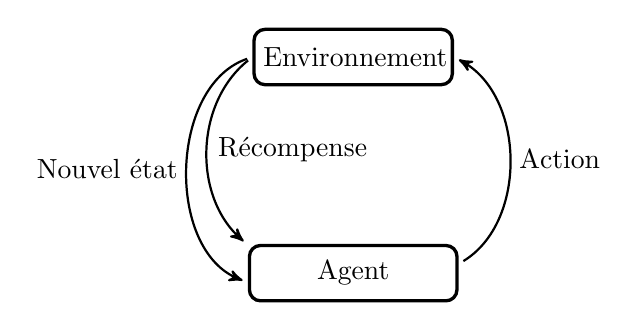
\begin{tikzpicture}[node distance=1cm, auto,]
         %nodes
          \node[punkt] (env) {Environnement};
          \node[punkt, inner sep=5pt,below=2cm of env]
          (agent) {Agent}
          edge[pilup,bend right=60] node[right] {Action} (env.east)
          edge[pildwn,bend left=70] node[left] {Nouvel état} (env.west)
          edge[pildwn,bend left=50] node[right] {Récompense} (env.west);
        \end{tikzpicture}
      \end{center}
      \caption{Principe d'apprentissage par renforcement}
      \label{fig:reinforcement_learning}
    \end{figure}
  \end{block}
\end{frame}

\section{Vie de l'agent, choix des actions et autres questions metaphysiques}
\begin{frame}[t]{Agent}
  \begin{block}{Definition}
    L'agent évolue dans son environnement. Il effectue des actions dans le but
    de maximiser l'espérance de récompense.
  \end{block}
\end{frame}
\begin{frame}[t]{Representation}
  \begin{block}{Esperances de recompenses}
    Stockées dans une matrice. Associe a un état et une action une espérance de
    récompense.
  \end{block}
\end{frame}

\section{Effectuer une action, conséquences}

\section{Évolution de l'agent, apprentissage}

\section{Conception modulaire}
\begin{frame}[t]{Séparation du code}
  \begin{block}{Inspiration}
    Calquée sur le jeu de tetris, un joueur et le jeu \(\rightarrow\)
    \texttt{agent} et \texttt{game}.
  \end{block}
\end{frame}

\section{Un agent, des agents?}
\end{document}
